\documentclass[conference]{IEEEtran}

\usepackage{amsfonts}
\usepackage{amsmath}
\usepackage[]{changepage}
\usepackage{float}
\usepackage[T1]{fontenc}
\usepackage[]{graphicx}
\usepackage[utf8]{inputenc}
\usepackage{makecell}
\usepackage{multirow}
\usepackage{pbox}
\usepackage{relsize}
\usepackage[group-separator={,}]{siunitx}
\usepackage{soul}
\usepackage{tabularx}
\usepackage{booktabs}
\usepackage{tabu}
\usepackage{cleveref}
\usepackage[normalem]{ulem}
\usepackage[table]{xcolor}
\usepackage{epigraph}

\newcommand{\conftitle}{2017 Conference on Scientific Analysis of Mobile Phone Datasets (NetMob)}

\usepackage{fancyhdr}
\chead{\conftitle}
\cfoot{\thepage}

\graphicspath{{../figures/}{./figures/}}

\DeclareMathOperator{\rank}{rank}
\DeclareMathOperator{\cov}{cov}

\bibliographystyle{plain}

\newcommand{\todo}[1]{\textbf{\color{red} TODO:\@ #1}}

\newcommand{\Beta}{B}
\newcommand{\mathA}{\mathcal{A}}
\newcommand{\mathB}{\mathcal{B}}
\newcommand{\mathC}{\mathcal{C}}
\newcommand{\mathG}{\mathcal{G}}
\newcommand{\mathP}{\mathcal{P}}

\newcommand{\TP}{\operatorname{TP}}
\newcommand{\TN}{\operatorname{TN}}
\newcommand{\FP}{\operatorname{FP}}
\newcommand{\TPR}{\operatorname{TPR}}
\newcommand{\FPR}{\operatorname{FPR}}
\newcommand{\AUC}{\operatorname{AUC}}

\newcommand{\closeopen}[2]{\left[ #1, #2 \right)}

% \title{Inference of Socioeconomic Status in a Communications Graph \\ A Bayesian Approach \\ \vspace{1ex} \Large{Extended Abstract}}

\title{Inference of Socioeconomic Status in a Communications Graph:  a Bayesian Approach}

\author{%
	\IEEEauthorblockN{%
	Martin Fixman\IEEEauthorrefmark{1}\IEEEauthorrefmark{2},
	Ariel Berenstein\IEEEauthorrefmark{1},
	Jorge Brea\IEEEauthorrefmark{1},
	Martin Minnoni\IEEEauthorrefmark{1},
	Matias Travizano\IEEEauthorrefmark{1},
	Carlos Sarraute\IEEEauthorrefmark{1}
	}
	\IEEEauthorblockA{\IEEEauthorrefmark{1}Grandata Labs, Bartolome Cruz 1818, Vicente Lopez, Argentina}
	\IEEEauthorblockA{\IEEEauthorrefmark{2}Universidad de Buenos Aires, Argentina}
	\IEEEauthorblockA{\{mfixman, ariel, jorge, martin, mat, charles\}@grandata.com}
}

\begin{document}

\maketitle

\begin{abstract}
Obtaining and processing demographical and sociological data have been some of the most important processes for understanding population-wide phenomena since at least 17th century~\cite{friendly2006}, and finding simple and intuitive ways of visualizing them has a big impact in our ways of understanding the data~\cite{minard1844,snow1855}. Common ways of obtaining useful qualitative data on socioeconomic stratification usually involved archival research or social surveys~\cite{bulmer1977}; however those methods can't present data that's at the same time exact, up to date, and that applies to a large population without having to rely on statistical methods.

Telecommunication operators (``telcos'') have access to a wealth of information about their users' communications and habits~\cite{huurdeman2003}, but the ability to store and process that data has taken large strides in the last few years thanks to new and more powerful computers and data mining techniques. The same can be said for sociological and economic information owned by banks and credit cards, and the relation between these two data sources.

Large scale data mining of data from the telecommunications industry is a relatively new area that's been so far mostly used for internal applications~\cite{han2002emerging}, but the gigantic wealth of real-time sociological data has been of interest for academic purposes related to sociology. This thesis builds on methods used by Óskardottir et.\ al.~\cite{oskardottir2016} and Singh et.\ al~\cite{singh2013predicting}, along with a large dataset of information for a certain telco and a large bank to find that the income distribution of the users follows closely (but not exactly) the income distribution of the whole population.

There's a strong homophily between the incomes of contacts in the telco, which along with the uneven distribution of wealth in the population is leveraged to create a methodology, grounded in Bayesian statistics, to infer socioeconomic level of a large subset of users in the network without banking information which is very accurate at $\AUC = 0.746$. The Bayesian method is later compared to several other methods based on supervised machine learning to prove that, even though it uses less input information, it's a better predictor of social features in this particular kind of network.

% In this work, we examine the socio-economic correlations present among users in a mobile phone network. First, we find that the distribution of income for a subset of users, for which we have income information given by a large bank, follows closely, but not exactly, the income distribution for the whole population. We also show the existence of a strong socio-economic homophily in the mobile phone network, where users linked in the network are more likely to have similar income. The main contribution of this work is that we leverage this homophily in order to propose a methodology, based on Bayesian statistics, to infer the socio-economic status for a large subset of users in the network (for which we have no banking information). With our proposed algorithm, we create an estimator for two categories (low and high income) which significantly outperforms both a simpler method based on a frequentist approach and several common \emph{Machine Learning} methods.

\end{abstract}

% !TEX root = tesis.tex

\chapter{Introduction}

% MOTIVATION
\section{Motivation of the Thesis}

In recent years, we have witnessed an exponential growth in the capacity to gather, store and manipulate massive amounts of data across a broad spectrum of disciplines: in astrophysics our capacity to gather and analyze massive datasets from astronomical observations has significantly transformed our capacity to model the dynamics of our cosmos; in sociology our capacity to track and study traits from individuals within a population of millions is allowing us to create social models at multiple scales, tracking individual and collective behavior both in space and time, with a granularity not even imagined twenty years ago.

In particular, mobile phone datasets provide a very rich view into the social interactions and the physical movements of large segments of a population. The voice calls and text messages exchanged between people, together with the call locations (recorded through cell tower usages), allow us to construct a rich social graph which can give us interesting insights on the users' social fabric, detailing not only particular social relationships and traits, but also regular patterns of behavior both in space and time, such as their daily and weekly mobility patterns~\cite{gonzalez2008understanding,ponieman2013human,sarraute2015city}.

Demographic factors play an important role in the constitution and preservation of social links. In particular concerning their age, individuals have a tendency to
establish links with others of similar age. This phenomenon is called age homophily~\cite{mcpherson2001birds}, and has been verified in mobile phone communications graph~\cite{blumenstock2010mobile,sarraute2014} as well as the Facebook graph~\cite{ugander2011anatomy}.


% PREVIOUS WORK ON THIS PROBLEM

Economic factors are also believed to have a determining role in both the social network's structure and dynamics. However, there are still very few large-scale quantitative analyses on the interplay between economic status of individuals and their social network. In~\cite{leo2015socioeconomic}, the authors analyze the correlations between mobile phone data and banking transaction information, revealing the existence of social stratification. They also show the presence of socioeconomic homophily among the networks participants using users' income, purchasing power and debt as indicators.
The authors of \cite{Luo2017inferring} studied the correlation between the position of a node in a mobile phone communications graph and its socio-economic status. They showed that the position and topological attributes in the graph can be used to generate inferences of the users' financial status.
In particular the study \cite{Luo2017inferring} shows the value of the Collective Influence~\cite{morone2015influence} as a topological attribute for the prediction of individual financial status.


% SUMMARY OF THE NEW APPROACH
\section{Summary of our Approach}

In this work, we leverage the socioeconomic homophily present in the cellular phone network to generate inferences of socioeconomic status in the communication graph. To this aim we will use the following data sources: (i) the Call Detail Records (CDRs) from the operator allow us to construct a social graph and to establish social affinities among users; (ii) banking reported income for a subset of their clients obtained from a large bank data source. We then construct an inferential algorithm that allows us to predict the socioeconomic status of users close to those for which we have banking information. To our knowledge, this is the first time both mobile phone and banking information has been integrated in this way to make inferences based on a social telecommunication graph.
Part of this work was published in~\cite{Fixman2016bayesian}.

The work done on this thesis is based the hypotheses that there is a significant level of homophily between a person's socioeconomic level and the one from its contacts (\cref{subsec:income_homophily}), and that using this correlation we can infer the first from the second (\cref{subsec:prediction_algorithm}).
At the same time, this thesis presents several ``conventional'' Machine Learning algorithms (\cref{sec:comparison}) along with an inference algorithm based in Bayesian Inference which works thanks to the correlation hypothesis (\cref{sec:inference_methodology}). This extra information should give this algorithm better results than the conventional ones.

Multiple strategies can be used to generate network features based on the CDRs. For instance, in \cite{oskarsdottir2016} the authors evaluate different collective inference methods applied to the churn prediction problem. Furthermore, the work \cite{oskarsdottir2017social} studies the impact of the social graph definition on the performance of the prediction methods. This motives the second part of the thesis, where we perform a comparative study of methods to generate network features for the nodes in the communication graph, and evaluate their impact on the inference of the income. We also compare the effectiveness of machine learning methods such as Logistic Regression and Random Forest on the different feature sets.

\todo{Add a summary of results}

\section{Organisation of the Thesis}

The remainder of the thesis is organized as follows.
In Chapter~\ref{chap:theoretical_intro} we provide an introduction to the theoretical ideas used in the thesis: the concept of homophily in social networks, \todo{complete}.

In Chapter~\ref{chap:related_work} we review related work on correlations in social-economic networks and on relation between socioeconomic status and mobile phone use. ETC \todo{complete}.

Chapter~\ref{sec:dataset} reviews the data sources used in this study. \todo{complete}.





\section{Experimental Dataset}

\subsection{Mobile Phone Data Source}
\label{subsec:mobiledatasource}

The data used in this study consist of a set \( \mathP \) of \textit{Call Detail Records} (CDRs), composed of voice calls and text messages from a Mexican telecommunication company (\textit{telco}) for a 3 month period.

Every CDR \( p \in \mathP \) contains the phone numbers of the caller and callee \( \left< p_o, p_d \right> \), which are anonymized using a cryptographic hash function for privacy reasons, the starting time \( p_t \), and, in the case of voice calls, the call duration \( p_s \). The latitude and longitude of the antenna used for each call \( \left< p_y, p_x \right> \) are also given for a subset of the data.

Given that our collection \( \mathP \) of CDRs are coming from one telephone company, we are able to reconstruct all communication links between clients of this company, as well as communications between the clients and other users, but we have no information on communications where neither users are clients of our telco company.

If we define \( N \) as the set of clients of the telco, and \( \mathP_N \subseteq \mathP \) as the calls where \( \forall p \in \mathP_N, \; p_o \in N \wedge p_d \in N \), we create a communications graph \( \mathG_N \) which contains only the users from the telco, and all the calls exchanged between them.

\todo{Add data where we include the time and SMS (?) of each call.}

\todo{Explain telco vs non-telco}

\todo{Separate into $P$ for calls and $S$ for SMS}

%With the data provided to us by the telco, \( \mathG \) contains \num{72107108} users who made \num{72107108} calls and sent \num{634225740} text messages in this period of 3 months.

\subsection{Banking Information}

For this study we also used account balances for over 10 million clients of a bank in Mexico for a period of 6 months, denoted \( \mathB \). The data for each client \( b \in \mathB \) contains his phone number \( b_p \), anonymized with the same hash function used in \( \mathP \), and the reported income of this person over 6 months \( b_{s_0}, \ldots, b_{s_5} \). We average these 6 values to get \( b_s \), an estimate of a user's income.

The bank also provided us demographic information for a subset of its clients \( \mathA \subseteq \mathB \). For each user \( u \in \mathA \), we are given the age \( u_a \) of the user, which allows us to observe differences in the income distribution according to the age. In another line of work, homophily with respect to age has been observed and used to generate inferences~\cite{brea2014}.

\begin{figure}[h]
\begin{center}
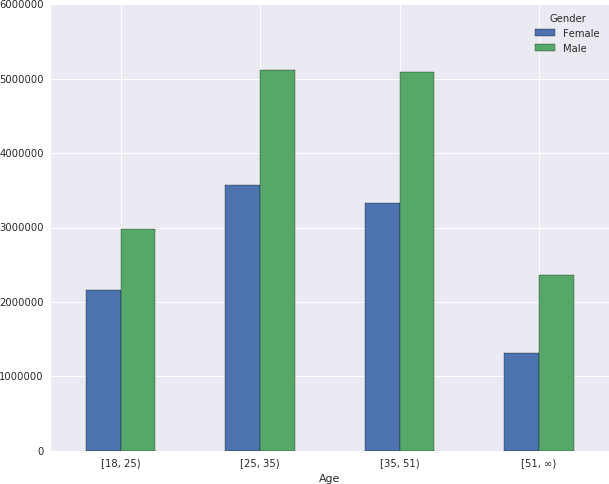
\includegraphics[width=0.9\columnwidth]{figures/gender_age_bar3/gender_age_bar3.png}
\caption{Amount of users in \( \mathB \) by gender and age.}
\label{gender_age_bar}
\end{center}
\end{figure}

\begin{figure}[h]
\begin{center}
{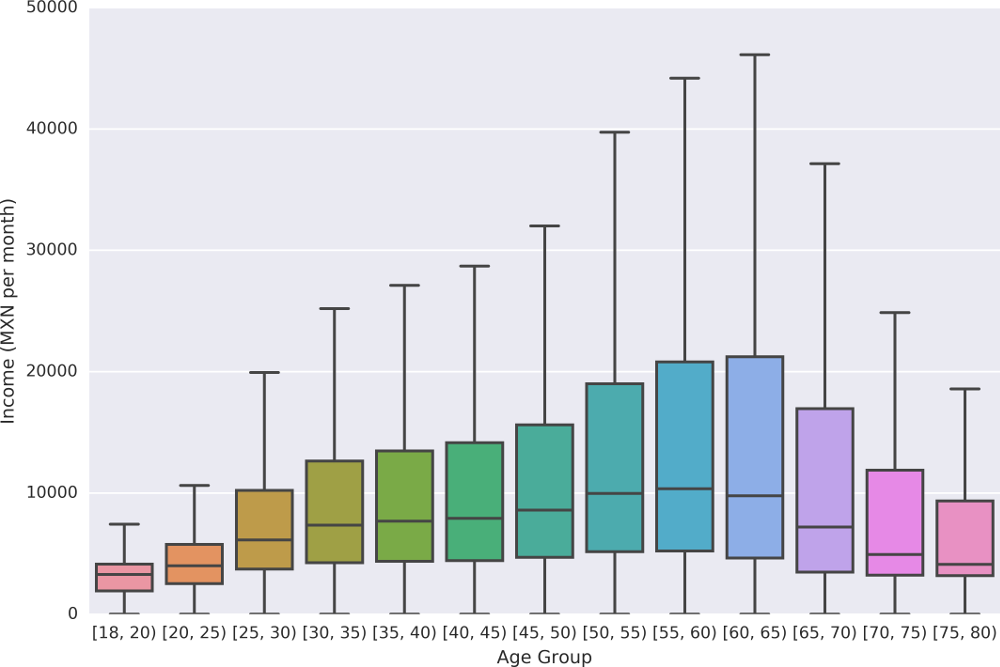
\includegraphics[width=0.9\columnwidth]{figures/income_age_boxplot4/income_age_boxplot4.png}}
\caption{Distribution of income \( b_s \) as a factor of age \( b_a \). This is consistent with data from median house income in Mexico~\cite{gallup2013}.}
\label{income_age_boxplot}
\end{center}
\end{figure}

\Cref{gender_age_bar} shows the distribution of users in \( \mathB \), according to their age range and gender.
\Cref{income_age_boxplot} shows the distribution of income, according to the age range (generated by taking 5 years intervals for the age).
It is interesting to note how the median income increases with the age, up to
the 60--65 years range (the retirement age in Mexico). After 65 years old, the median income rapidly decreases.

\subsection{Bank and Telco Matching}

Since the phone numbers in each call \( p_o \) and \( p_d \) are anonymized with the same hash function as the phone number in the bank data, \( b_p \), we can match users to their unique phone to create the social graph (\( \bowtie \) denotes the inner join operator).

\begin{equation}
G = \mathP \bowtie_{_{p_o = b_p}} \mathB \bowtie_{_{p_d = b_p}} \mathB
\label{join}
\end{equation}

\( G \) includes income information for the subset of the social graph that appears in the bank data, so \( \forall g \in G \) we have its phone number \( g_p \), its average income over 6 months \( g_s \), and its age \( g_a \).
This graph has a total of \num{2027554} nodes with \num{5044976} edges, which represent \num{29599762} calls and \num{5476783} text messages.

\subsection{Outlier Filtering}

The dataset contains information about bank and telco users, some of which may not directly correspond to a human user, % who exclusively users the telco and the bank used in this study,
or may not have useful information for our research.
Most of the telco users in the first case are already filtered by the intersection (\textsc{inner join}). To make sure the users are relevant enough for this study, we only keep the users which have:

\begin{itemize}
	\item More than 5 calls in either direction.
	\item A monthly income of at least \$\num{1000}.
	The value is expressed in Mexican pesos (MXN)\footnote{At the time of writing (July 14, 2016), 1000 Mexican pesos are equivalent to 54 US dollars.}.
	\item A monthly income in the \num{99}th percentile (i.e.\ we filter users with a monthly income in the top 1\%).
\end{itemize}

\subsection{Unequal Distribution of Income}

We provide here some observations of the distribution of income of the bank clients. These observations correspond to the filtered dataset, obtained after applying the filters of the previous section.

\Cref{fig:income_distribution} shows the Lorenz curve, graphical representation of the distribution of income. The X axis plots the cumulative share of clients, ordered from lowest to highest incomes. The Y axis plots the fraction of the total income that they have.

\begin{figure}[ht]
\begin{center}
{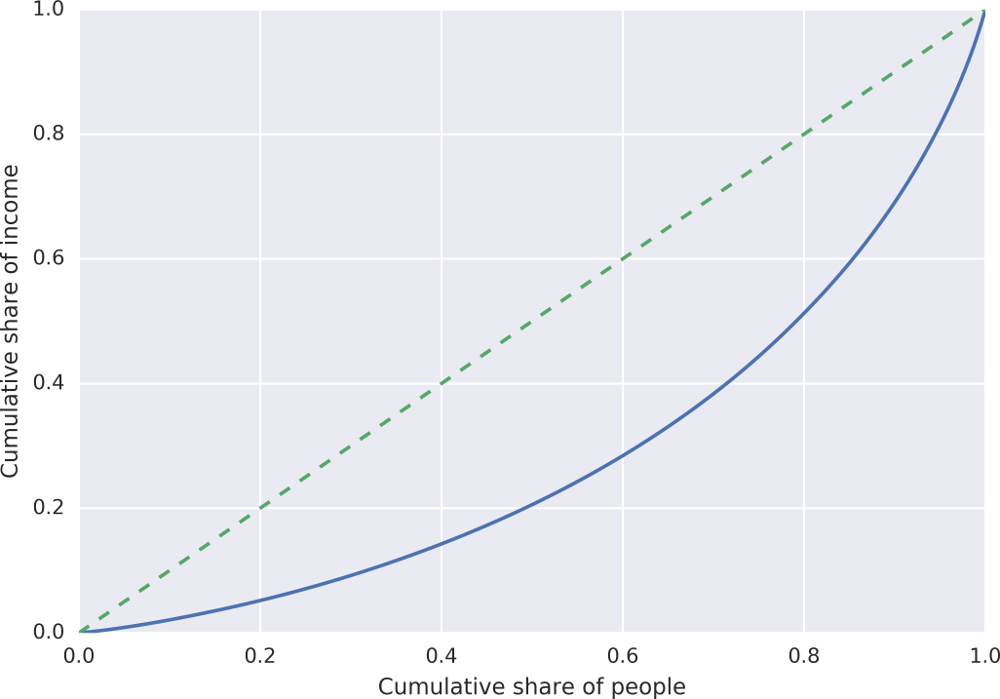
\includegraphics[width=0.9\columnwidth]{figures/cumulative_income.png}}
\caption{Lorenz curve representing the distribution of income of bank clients.}
\label{fig:income_distribution}
\end{center}
\end{figure}

From the Lorenz curve, we can compute the Gini coefficient, as the area that lies between the line of perfect equality (the line at \( 45^{\circ} \)) and the Lorenz curve over the total area under the line of equality.
The Gini coefficient obtained is \( G = 0.45 \).

According to the World Bank~\cite{world_bank}, the Gini coefficient for the whole population of Mexico was 0.481 in 2012. Our result is consistent with this information, since the income inequality is expected to be lower within the bank clients than within the whole population of the country.

Looking at the cumulative share of the clients with highest incomes, we observe that the top 10\% of clients accumulate 33\% of the total income; the top 20\% accumulate 50.5\%; and the top 30\% accumulate 63.1\% of the total income.

% \todo{Distribution per region.}
% \todo{Comparison with statistics from Mexico.}

 
\section{The Bayesian Method}
\label{sec:inference_methodology}

\subsection{Income Homophily}
\label{subsec:income_homophily}

\begin{figure}
\centering
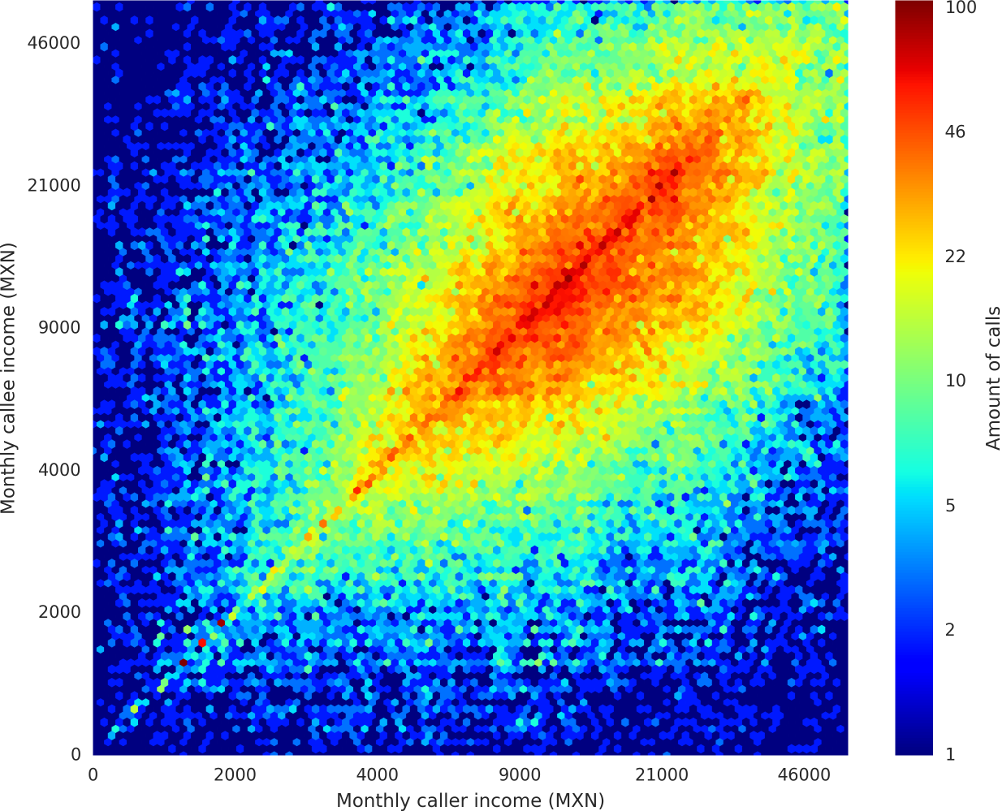
\includegraphics[width=\columnwidth]{figures/Homophily_income_origin_target_1/Homophily_income_origin_target_1.png}
\caption{Heatmap showing the number of calls between users, according to their monthly income. There is a higher probability that the callee and the caller have similar income levels.}
\label{fig:homophily_heatmap}
\end{figure}

The main contribution of this work is the estimation of the income of the telco users for which we lack banking data, but have bank clients in their neighborhood of the network graph. To show the feasibility of this task, we first show the existence of a strong income homophily in the telco graph as is evidenced in \Cref{fig:homophily_heatmap}.

For each pair $\left\{ \left< p_o, p_d \right> \mid p \in P \right\}$, the X coordinate is defined as the set of incomes for callers, while the Y coordinate is the set of incomes for callees. According to what we can observe in \Cref{fig:homophily_heatmap}, there should be a significant correlation between $X$ and $Y$. Given the broad non-Gaussian distribution of the income's values, we choose to use a rank-based measure of correlation which is robust to outliers.

Namely, the \textit{Spearman's rank correlation}, as defined in defined in \Cref{spearman}, is computed to test the statistical dependence of sets of incomes of callers and callees. Applying this formula to the data gives a correlation coefficient of $\mathbf{r_s = 0.474}$.

The result was compared with a randomized null hypothesis, where links between users are selected randomly disregarding income data, obtaining a $p\text{-value}$ of $p < 10^{-6}$. These values for $r_s$ and $p$ show a strong indication of income homophily among users in our communication graph. This observation is consistent with the results reported in other investigation of similar data, namely~\cite{leo2015socioeconomic}.

We can take advantage of this homophily to propagate income information to the rest of our graph $P$, where the income of the complete set of users is unknown.

\subsection{Prediction Algorithm}
\label{subsec:prediction_algorithm}

\subsubsection{Discrimination by Wealth}
\label{subsec:discrimination_by_wealth}

The main objective of this research is to identify users with higher income. To make the task simpler and more efficient, the actual income values as described in \Cref{subsec:bank_source} are forfeited and instead the customers are separated into distinct groups: $H_1$, containing customers whose income is lower or equal than the median, and $H_2$, containing users whose income is higher than this value. From now on, these will be referred as \emph{Low Income} and \emph{High Income} users respectively.

The median value in the dataset, after accounting for outliers as explained in \Cref{subsec:outlier_filtering}, is of exactly \textbf{6300 MXN}. This way, we can define the two groups as in \Cref{eq:h}.

\begin{equation}
\label{eq:h}
\begin{gathered}
H_1 \cup H_2 = S \\
\left( \forall h \in H_1 \right) h_s \leq 6300 \\
\left( \forall h \in H_2 \right) h_s > 6300
\end{gathered}
\end{equation}

\subsubsection{Feature Accumulation}
\label{subsec:feature_accumulation}

Given the \emph{Social Graph} $G = \left< V, E \right>$, as defined in \Cref{sec:dataset}, contains information about the \emph{Calls}, \emph{SMS}, and \emph{Total Time} of each link between two users. These can be accumulated for each user, along with its \emph{Degree}, to produce the \emph{User Data}, which is used for another evaluation in \Cref{subsec:user_data}.

Another possible way to accumulate these values is discriminating them by the category to which the other endpoint belong. That is, for every edge feature $F$ and for the \emph{Degree}, it's possible to define two features $F_{\low}$ and $F_{\high}$ that only accumulate features from edges whose other endpoint is a user with \emph{Low Income} or \emph{High Income}, respectively. This approach is formalized in \Cref{eq:bayesian_accum}\maybe{Redo formulas so they look nicer}.

\begin{equation}
\label{eq:bayesian_accum}
\begin{gathered}
\begin{aligned}
& \calls^{\low}_v = \sum_{\substack{e \in E \\ e_d = v \\ e_o \in H_1}}{e_c} + \sum_{\substack{e \in E \\ e_o = v \\ e_d \in H_1}}{e_c}
& \calls^{\high}_v = \sum_{\substack{e \in E \\ e_d = v \\ e_o \in H_2}}{e_c} + \sum_{\substack{e \in E \\ e_o = v \\ e_d \in H_2}}{e_c} \\
& \etime^{\low}_v = \sum_{\substack{e \in E \\ e_d = v \\ e_o \in H_1}}{e_t} + \sum_{\substack{e \in E \\ e_o = v \\ e_d \in H_1}}{e_t}
& \etime^{\high}_v = \sum_{\substack{e \in E \\ e_d = v \\ e_o \in H_2}}{e_t} + \sum_{\substack{e \in E \\ e_o = v \\ e_d \in H_2}}{e_t} \\
& \sms^{\low}_v = \sum_{\substack{e \in E \\ e_d = v \\ e_o \in H_1}}{e_s} + \sum_{\substack{e \in E \\ e_o = v \\ e_d \in H_1}}{e_s}
& \sms^{\high}_v = \sum_{\substack{e \in E \\ e_d = v \\ e_o \in H_2}}{e_s} + \sum_{\substack{e \in E \\ e_o = v \\ e_d \in H_2}}{e_s}
\end{aligned} \\
\begin{aligned}
\contacts^{\low }_v &= c^{\low}_v &= &\left| \left\{ e \in E \; \middle| \begin{aligned} &e_o = v &\land &\quad e_d \in H_1 \\ &&\lor & \\ &e_d = v &\land &\quad e_o \in H_1 \end{aligned} \right\} \right| \\
\contacts^{\high}_v &= c^{\high}_v &= &\left| \left\{ e \in E \; \middle| \begin{aligned} &e_o = v &\land &\quad e_d \in H_2 \\ &&\lor & \\ &e_d = v &\land &\quad e_o \in H_2 \end{aligned} \right\} \right|
\end{aligned}
\end{gathered}
\end{equation}

\subsubsection{Uncertainty}
\label{subsec:uncertainty}

One important thing to note is that the only nodes accumulated in \Cref{eq:bayesian_accum} for some node $v \in V$ are the neighbouring ones that belong to $S$. \Cref{eq:subset_neighbours} indicates how to build the subset $D \subseteq S$ of bank users who also have a neughbour in the \emph{Social Graph} $G$ which is also part of the bank.

\begin{equation}
\label{eq:subset_neighbours}
\begin{gathered}
E^D = \left\{ e \in E \mid e_o \in S \land e_d \in S \right\} \\
D = E^D_o \cup E^D_d
\end{gathered}
\end{equation}

$D$ is defined as a subset of $S$, instead of one of $V$, because we cannot analyze the performance of a predictor on telco users who aren't part of the bank.

There is an additional level of uncertainty: while the data contains information about calls, and the inference assumes that callee and caller know each other (which is usually true after we remove outliers, as in \Cref{subsec:outlier}), there is simply no information about the socioeconomic level of acquaintances who don't share phone calls. However, the more calls a user names, and the more people it calls, the more \emph{Certain} we can be that the algorithm in this section is correct.

\subsubsection{Modelling Users}
\label{subsec:modelling_users}

The final objective of this thesis is to detect \emph{High Income} users in a dataset by just knowing their calls using the hypothesis, described in Section~\ref{subsec:income_homophily}, that a user will mostly call people from his same income category. For this, some calculated will be made on the low and high calculations for some property $\varpi$\footnotemark{}, which is one of the values defined in Equation~\ref{eq:property}. Part of the performance calculations in Section~\ref{sec:results} will imply finding the $\varpi$ which maximizes some score.

\footnotetext{$\varpi$ is a variant of the Greek letter $\pi$, which represents a \textbf{P}roperty.}

\begin{equation}
\label{eq:property}
\varpi \in \left\{ \calls, \etime, \sms, \contacts \right\}
\end{equation}

As it was discussed in Section~\ref{subsec:uncertainty}, even having that data it's impossible to have complete information about a user's relationships. However, it's possible to create a \emph{Model} where we can predict the rate of \emph{High Income} to \emph{Low Income} contacts a user has, and with that data the Probability $p_v$ that this user $v \in V \setminus B$ is a \emph{High Income} user.

The naïve way of solving this problem would be to assign this probability using only the current data, as in Equation~\ref{eq:naive_p}. However, this fails to account for the \emph{Certainty} that a user belongs to some category, which can be exemplified in scenarios where the probability of a user with only 1 \emph{High Income} contact being \emph{High Income} is slightly higher than one for another user with 100 \emph{High Income} contacts and 1 \emph{Low Income} contact.

\begin{equation}
\label{eq:naive_p}
p_v = P \left( v \in H_2 \right) = \frac{\varpi^{\high}_v}{\varpi^{\high}_v + \varpi^{\low}_v}
\end{equation}

A better way to define this model is to create, for each user $v \in V \setminus B$, a \emph{Beta Distribution} $\Beta_v$ which can define the probability of $p_v$ falling between two numbers. This approach is formalized in Equation~\ref{eq:beta}.

\begin{equation}
\label{eq:beta}
\begin{gathered}
p_v \sim \Beta \left( \varpi^{\high}_v + 1, \varpi^{\low}_v + 1 \right) \\
P \left( p_v \leq x \right) = \frac{1}{\Beta \left( \varpi^{\high} + 1, \varpi^{\low} + 1 \right)} \cdot \int_0^x {t^{\varpi^{\high}} {\left( 1 - t \right)}^{\varpi^{\low}} dt}
\end{gathered}
\end{equation}

Here it's also possible to assign the probability depending on the \emph{Mean} or the \emph{Mode} of the distribution. However, that would also fail to account for the \emph{Certainty} of the numbers.

Instead, given the definition of an arbitrary $\Theta$, initially defined as $\Theta = 0.005$\maybe{Make sure this is true}, it's possible to use the formula presented in Section~\ref{subsec:beta_ppf} to define a suitable $p_v$, as shown in Equation~\ref{eq:beta_theta_ppf}.

\todo{Test different $\Theta$s}

\begin{equation}
\label{eq:beta_theta_ppf}
\begin{aligned}
p_v &= Q \left (\Theta \right) \\
&= \inf \left\{ x \in \left[ 0, 1 \right] \mid \Theta \leq F(x) \right\}
\end{aligned}
\end{equation}

\subsubsection{Categorizing Users}

In the previous section the probability of belonging of being a \emph{High Income} user $p_v$ was defined for every $v \in V \setminus B$. While this value alone doesn't give any information about whether user $v$ belongs which category, it does tell that his category will be higher or equal than users with a lower probability. This approach is formalized in Equation~\ref{eq:pv_minus}.

\begin{equation}
\label{eq:pv_minus}
\begin{gathered}
\left( \forall u, w \in V \setminus B \right) \\
\begin{aligned}
p_u > p_w \land u \in H_1 &\implies w \in H_1 \\
p_u < p_w \land u \in H_2 &\implies w \in H_2 \\
p_u = p_w \implies ( u \in H_1 &\iff w \in H_1 )
\end{aligned}
\end{gathered}
\end{equation}

Thanks to this approach we can define some limit, $\tau$, and categorize each user $v \in V \setminus B$ as either category depending on the magnitude of $p_v$ compared to $\tau$, as in Equation~\ref{eq:pv_tau}.

\begin{equation}
\label{eq:pv_tau}
\begin{aligned}
p_v \leq \tau &\implies v \in H_1 \\
p_v > \tau &\implies v \in H_2
\end{aligned}
\end{equation}

\subsubsection{Performance Evaluation}
\label{subsec:performance_evaluation}

It's easy to evaluate the performance by calculating $p_v$ for all $v \in B$, which allows us to know whether each value is a \emph{True~Positive}, a \emph{False~Positive}, a \emph{False~Negative}, or a \emph{True~Negative}, and collecting any of the metrics described in Section~\ref{subsec:mlmetrics}.

One advantage of this method is that it's possible to evaluate the method by calculating the \emph{Area Under the Curve} without having to specify a particular $tau$, since this follows the necessary pattern defined in Section~\ref{subsec:auc}. This way it's possible to select the best $\varpi$ without having to select the respective $\tau$.

Additionally, after defining a $\varpi$, it's easy to select a $\tau$ so that the final \emph{Accuracy} is maximized.

% We define the set \( Q \) as the group of users having at least one connection link to bank clients. For each user \( q^j \in Q \), we compute the number of outgoing calls \( a^j_i \) to the category \( H_i \). Our hypothesis, given the observed homophily, is that if a user \( q^j \) has a higher number of calls \( a^j_i \) to the category \( H_i \) than the other category, it would be more likely to belong to the \( H_i \) income category. In other words, a person is usually in the same income category as the majority of people it calls.

% A straightforward approach would be to define the income category of a user as the category where most of its contacts belong. The problem with this approach is that it does not factor in the higher uncertainty in our estimates for users with fewer calls. To address this uncertainty, instead of using calling frequencies to define the probability of a user belonging to the high income category, we use the amount of calls \( a^j_i \) as parameters defining a Beta distribution for the probability of belonging to a given category. We have therefore taken a Bayesian rather than a frequentist approach to income prediction.

% We define \(\Beta^j\) as the Beta probability distribution function for each user, which defines a distinct distribution for each user. Having obtained the Beta distribution for the probability of belonging to the high income category, we then find the lowest 5\textsuperscript{th} percentile \( p_{\operatorname{lower}} \) for this probability. If \( p_{\operatorname{lower}} \) is above a given threshold \( \tau \), we set the user's income to \( H_2 \), otherwise we set his income category to \( H_1 \). We note that this criteria takes into account both the mean and the broadness (uncertainty) of the distribution. We also note that the category assigned to a user depends not only on its Beta distribution but also on our choice of \( \tau \).

%We therefore choose a value for \( \tau \) which maximizes the trade off between true positive (\( TPR \)) and false positive (\( FPR \)) rates: \( TPR=TP/P \) and \( FPR=FP/N \) where \( TP \) is the number of correctly predicted users with high income, \( P \) is the total number of users with high income, \( FP \) is the number of users incorrectly classified as having high income, and \( N \) is the total number of users with low income.

%For each user \( q^j \) we estimate and the corresIn this way we obtained a Dirichlet distribution for each user \( q^j \) and compute

%According to the Dirichlet Distibution, each user has a caller income category probability density function of the form

%For all the other users in the telco having at least one link to any other telco user with a defined income \( q \in Q = \left\{x \in \left( N \setminus B \right) \mid (\exists y \in G) \left< x, y \right> \in P \vee \left< y, x \right> \in P \right\} \), we can use this distribution to infer the probabilities of being part of each group \( H_1, \ldots, H_5 \), and this way approximate the economic status.

 
\section{Evaluating Performance}
\label{sec:results}

In this section, we test the \emph{Prediction Algorithm} presented in Section~\ref{subsec:prediction_algorithm} with the data present on the graph.

\subsection{Data Partitioning}

\subsubsection{Train Test Split}
\label{subsec:train_test_split}

As with many other classification problems, the \emph{Bayesian Algorithm} is prone to overfitting~\cite{mitchellml1997}. In this particular case, since the information presented in Section~\ref{subsec:income_homophily} shows that users tend to communicated with users of the same socioeconomic level, by running the algorithm in the complete data and using the same users as part of the features and of the labels, we would erroneously be having more data per user than we would have when modelling the problem.

An easy way to avoid this problem is by doing a simple \emph{Train Test Split}, where the data in $B$ is separated into two disjoint groups, $B = B_{\train} \cup B_{\test}$ and $B_{\train} \cap B_{\test} = \varnothing$, where $\left| B_{\train} \right| = \sfrac{4}{5} \cdot \left| B \right|$ and $\left| B_{\test} \right| = \sfrac{1}{5} \cdot \left| B \right|$.

\subsubsection{Erasing Uninformative Data}

Given that $\left| B \right| \ll \left| V \right|$ and that $G$ is sparse, the vast majority of users don't have any kind of contact with users of the bank. For this reason it's useless to evaluate the performance of the algorithm using all the nodes, and therefore the \emph{Testing Set} used in this thesis will instead focus on the bank users that have at least one contact with another bank user. This approach is formalized in Equation~\ref{eq:inner_graph}.

\begin{equation}
\label{eq:inner_graph}
\begin{gathered}
\hat{E} = \left\{ e \in E \mid e_o \in B_{\train} \lor e_d \in B_{\train} \right\} \\
\hat{B}_{\test} = B_{\test} \cap \left( \hat{E}_o \cup \hat{E}_d \right)
\end{gathered}
\end{equation}

This approach works perfectly when $\varpi = \contacts$. However, it's possible that for other values of $\varpi$ there won't be any information available in $\hat{B}_{\test}$ in the case of users who either didn't receive any call from a bank user or didn't receive any message.

The equations~\ref{eq:inner_graph_call} and~\ref{eq:inner_graph_sms} formalize new variables to use for informative data in those cases.

\begin{equation}
\label{eq:inner_graph_call}
\begin{gathered}
\hat{E}^{\calls} = \left\{ e \in E \mid e_c > 0 \land \left( e_o \in B_{\train} \lor e_d \in B_{\train} \right) \right\} \\
\hat{B}^{\calls}_{\test} = B_{\test} \cap \left( \hat{E}^{\calls}_o \cup \hat{E}^{\calls}_d \right) \\
\end{gathered}
\end{equation}

\begin{equation}
\label{eq:inner_graph_sms}
\begin{gathered}
\hat{E}^{\sms} = \left\{ e \in E \mid e_s > 0 \land \left( e_o \in B_{\train} \lor e_d \in B_{\train} \right) \right\} \\
\hat{B}^{\sms}_{\test} = B_{\test} \cap \left( \hat{E}^{\sms}_o \cup \hat{E}^{\sms}_d \right)
\end{gathered}
\end{equation}

\subsubsection{Rebalancing Labels}
\label{subsec:rebalancing_labels}

Since the testing data $B_{\test}$ was a random subsample of a balanced set (see Section~\ref{subsec:train_test_split} and Section~\ref{subsec:discrimination_by_wealth}), it was also balanced itself\maybe{Make sure $B$ refers only to bank users \textbf{in the telco}}. However, since \emph{High Income} users tend to communicate more often than \emph{Low Income} ones, $\hat{B}_{\test}$ is unbalanced and has a significant bias for high-income users.

Since the income categories tend to be balanced in the real world, this isn't wanted. However, since it's not necessary to use the entire \emph{Testing Set} for testing the algorithm, a simple way would be to create a new, balanced, and final testing set, $\Upsilon \subseteq \hat{B}_{\test}$ containing all users from $\hat{B}_{\test}$ \emph{Low Income}, along with a random sample of the same size with \emph{High Income}.

\begin{equation}
\label{eq:upsilon}
\begin{gathered}
\begin{aligned}
\Upsilon^{\low} &= \hat{B}_{\test} \cap H_1 \\
\Upsilon^{\high} &\subseteq \hat{B}_{\test} \cap H_2
\end{aligned} \\
\left| \Upsilon^{\low} \right| = \left| \Upsilon^{\high} \right| \\
\Upsilon = \Upsilon^{\low} \cup \Upsilon^{\high}
\end{gathered}
\end{equation}

$\Upsilon$ will be the only \emph{Testing Set} used from now on, while $B_{\train}$ will be used as training set.

Additionally, the sets $\Upsilon^{\calls}$ and $\Upsilon^{\sms}$ refer to similar sets which are taken from users from the \emph{Testing Set} that had at least one call or sent at least one SMS, respectively, to another user in the \emph{Training Set}.

\subsubsection{Set Magnitudes}

While the new set $\Upsilon$ contains significantly less users than the original set $B$, it still has a sufficient amount of people to make a prediction. Table~\ref{tab:partition_numbers} shows the number of users that remain after every trim used in this Subsection, along with the ratio of users which we would be able to assign an \emph{Income Category} using these datasets assuming the real data is equally distributed from the \emph{Test Data}.

\begin{table}
\centering
\begin{tabular}{l r r r c}
\toprule
Set & Total Size & High Income & Low Income & Ratio \\
\midrule
$B$ & \num{5402959} & \num{2702628} & \num{2700331} & \NA{} \\
$B_{\test}$ & \num{1080592} & \num{540526} & \num{540066} & \NA{} \\
$\hat{B}_{\test}$ & \num{53691} & \num{35215} & \num{18476} & \num{1.000} \\
$\Upsilon$ & \num{36952} & \num{18476} & \num{18476} & 1.000 \\
$\Upsilon^{\calls}$ & \num{30715} & \num{15653} & \num{15062} & 0.831 \\
$\Upsilon^{\sms}$ & \num{11909} & \num{6046} & \num{5863} & 0.322 \\
\bottomrule
\end{tabular}
\caption{Amount of users in the \emph{Testing Set} after trimming it several times to prevent overfitting while keeping the labels balanced}
\label{tab:partition_numbers}
\end{table}

\subsection{Algorithm Performance on All Users}
\label{subsec:algorithm_performance}

The \emph{Bayesian Algorithm} will be ran for every $\varpi \in \left\{ \contacts, \calls, \etime, \sms \right\}$. For every possible configuration, we present 3 plots for $\Theta = 0.005$.

\begin{itemize}
	\item A \textbf{histogram} presenting the distribution of the $p_v$ values which result from applying Equation~\ref{eq:beta_theta_ppf} presented in Section~\ref{subsec:modelling_users} to each distinct \emph{Beta Distribution}.
	\item An \textbf{Receiver Operating Characteristic Curve}, showing the tradeoff of \emph{False Positive Rate} to \emph{True Positive Rate} when selecting every possible $\tau$. The \emph{Area Under the Curve} is marked, as this is the metric that is being maximized when selecting the correct $\varpi$.
	\item An \textbf{Accuracy Curve}, which shows the \emph{Accuracy} of the predictor by its \emph{False Positive Rate}. $\tau$ is chosen as to maximize this value.
\end{itemize}

\subsubsection{Inferring by Calls}
\label{subsec:calls_infer}

\begin{center}
\includegraphics[width=\textwidth]{figures/bayes/hist_calls.png}
\includegraphics[width=.49\textwidth]{figures/bayes/roc_calls.png}
\includegraphics[width=.49\textwidth]{figures/bayes/accuracy_calls.png}
\end{center}

When $\varpi = \calls$ and the data is analyzed using $\Upsilon^{\calls}$ as \emph{Testing Set}, the \emph{Inverse Cumulative Distribution Function} has several peaks containing groups of users with similar amount of calls, and the data has a significant bias towards calls towards calls to \emph{Low Income} users.

After analyszing the data, we find that the \emph{Area Under the Curve} using this method is of \num{0.721}, which is significantly higher than all the naïve and \emph{Machine Learning} methods presented in the later Section~\ref{sec:comparison}.

To maximize accuracy, setting $\tau = 0.224$ results in a predictor where $\Accuracy = 0.684$ and $\FPR = 123$. Additionally, that value of $\tau$ results in $\Precision = 123$, $\Recall = 123$, $F_1 = 123$, and $F_4 = 123$. \todo{Fill these values.}

\subsubsection{Inferring by Time}
\label{subsec:time_infer}

\begin{center}
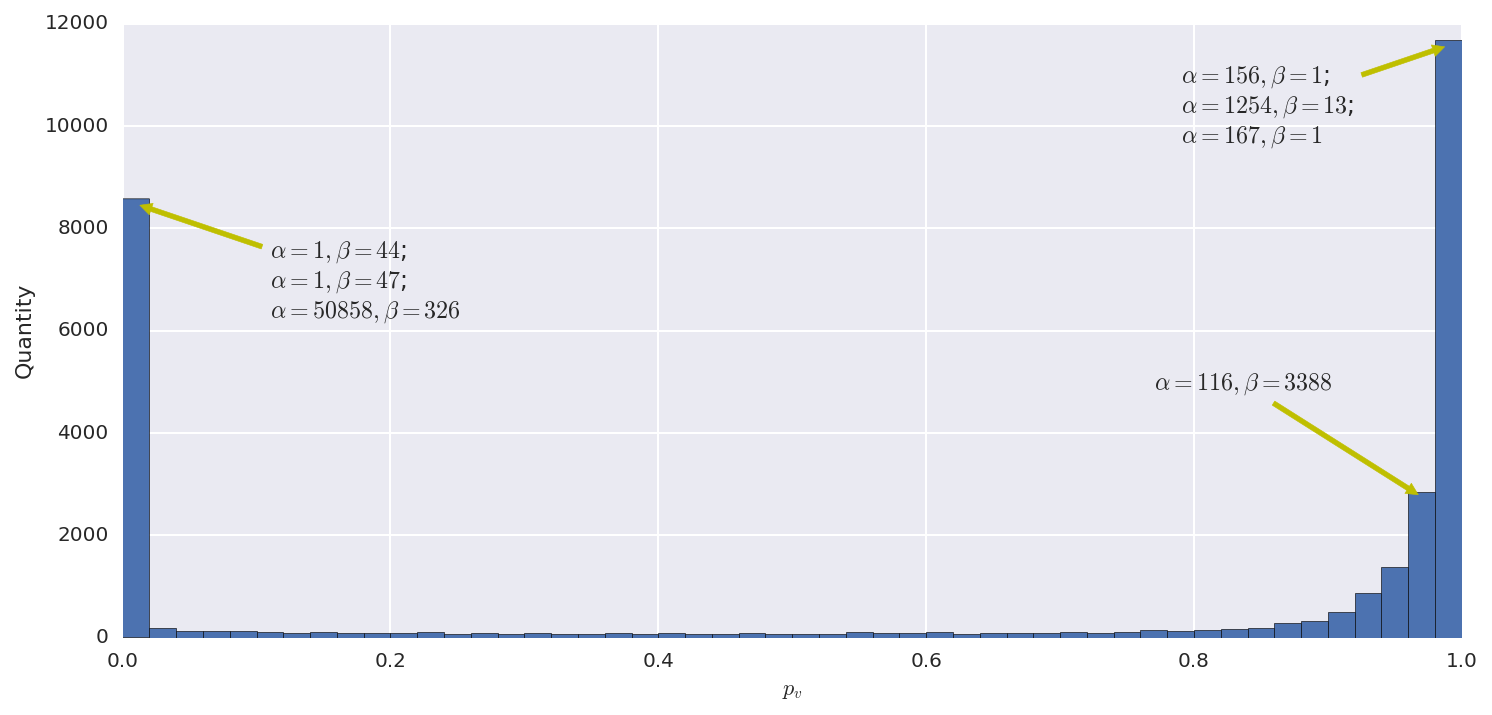
\includegraphics[width=\textwidth]{figures/bayes/hist_time.png}
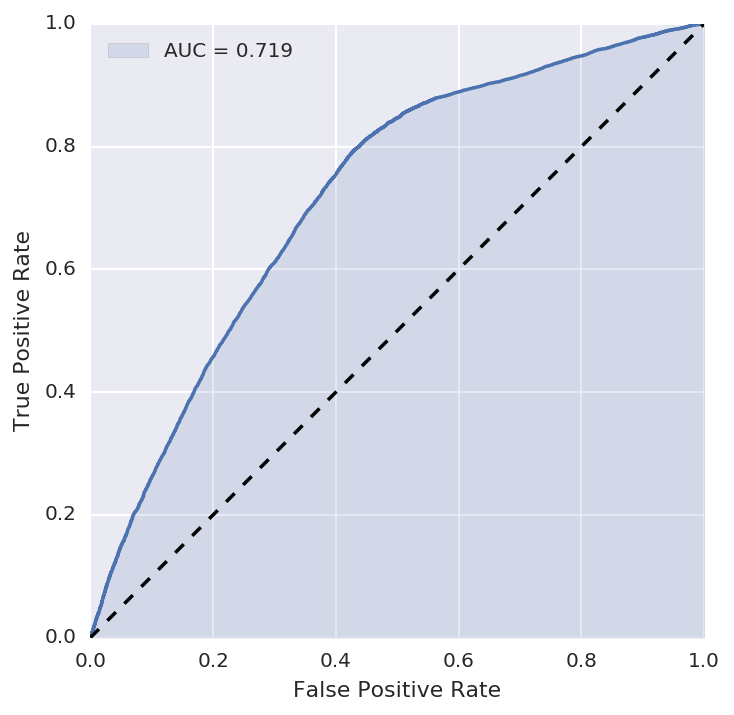
\includegraphics[width=.49\textwidth]{figures/bayes/roc_time.png}
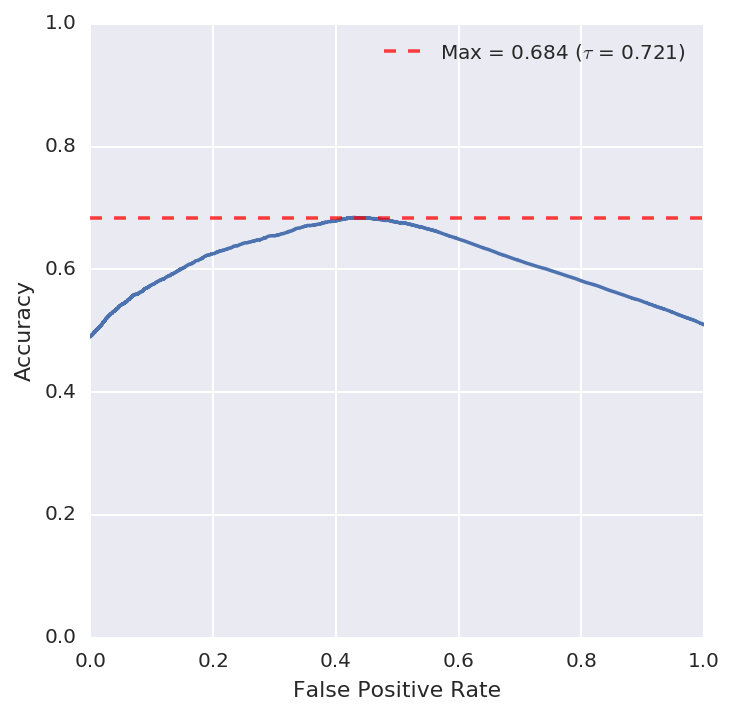
\includegraphics[width=.49\textwidth]{figures/bayes/accuracy_time.png}
\end{center}

When $\varpi = \etime$ and the data is analyzed using $\Upsilon^{\calls}$ as \emph{Testing Set}, there are two big clusters of data at the edges. The reason for these is that, as shown by Figure~\ref{fig:timeheatmap}, the majority of users only call either \emph{High Income} or \emph{Low Income} users. For completeness sake, this test is run again in Section~\ref{fig:time_infer_positive} only for the subset $\hat{\Upsilon}^{\calls} \subseteq \Upsilon^{\calls}$ which have at least one call to users of each income category; however, while this makes the histogram more equitative taking out the users with SMS to both categories (whose users tend to be in that same category) makes all the metrics lower.

The \emph{Area Under the Curve} of this inference mechanism is $\AUC = 0.719$, which is lower than the one for the calls in Section~\ref{subsec:call_infer}. The \emph{Accuracy Curve} is unsurprisingly similar to that one, and even the \emph{Accuracy} at $\tau = 0.721$ is the same. This is probably a result of using the same dataset as that section, and the fact that there is an obvious correlation between total talking time and total calls, shown in Figure~\ref{fig:call_time}.

That value of $\tau$ also results in a predictor where $\Accuracy = 0.684$, $\FPR = 123$, $\Precision = 123$, $\Recall = 123$, $F_1 = 123$, and $F_4 = 123$. \todo{Fill these values.}

\subsubsection{Inferring by SMS}
\label{subsec:sms_infer}

\begin{center}
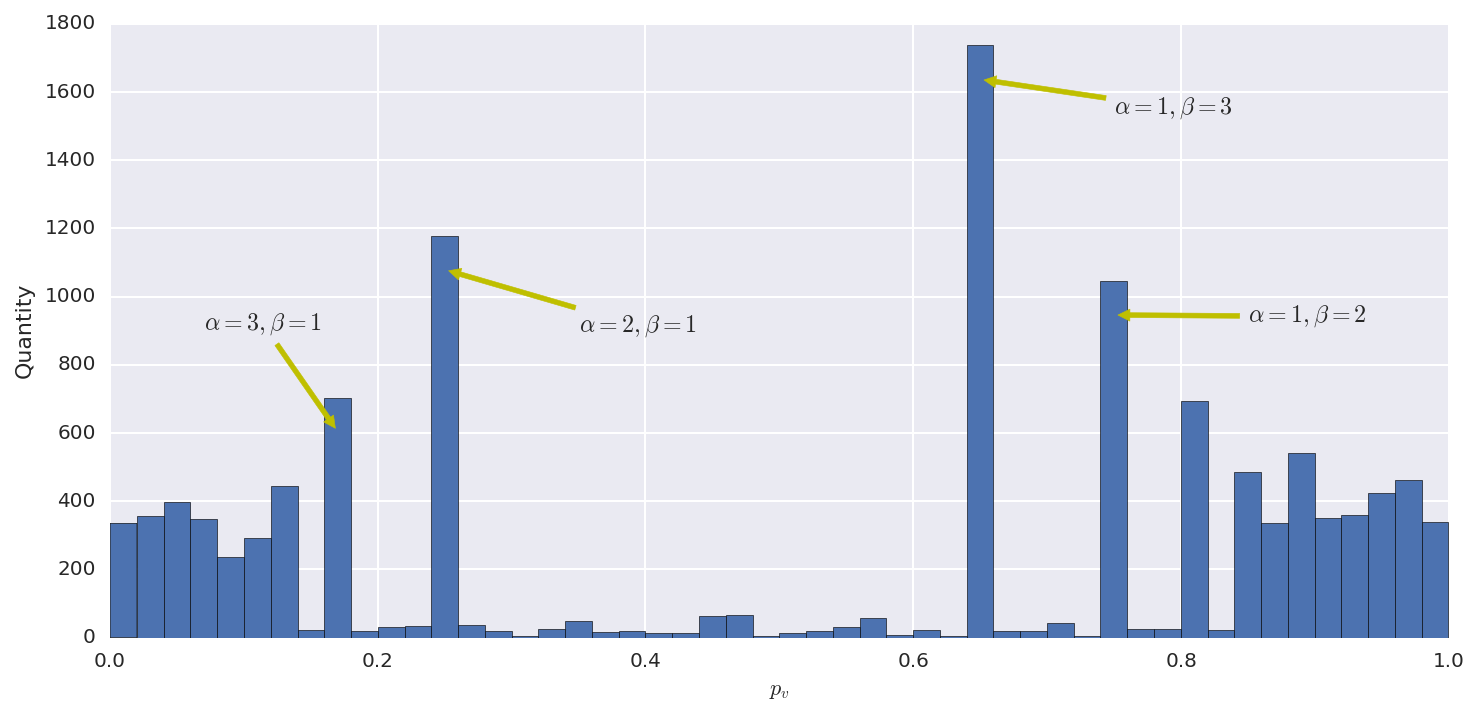
\includegraphics[width=\textwidth]{figures/bayes/hist_sms.png}
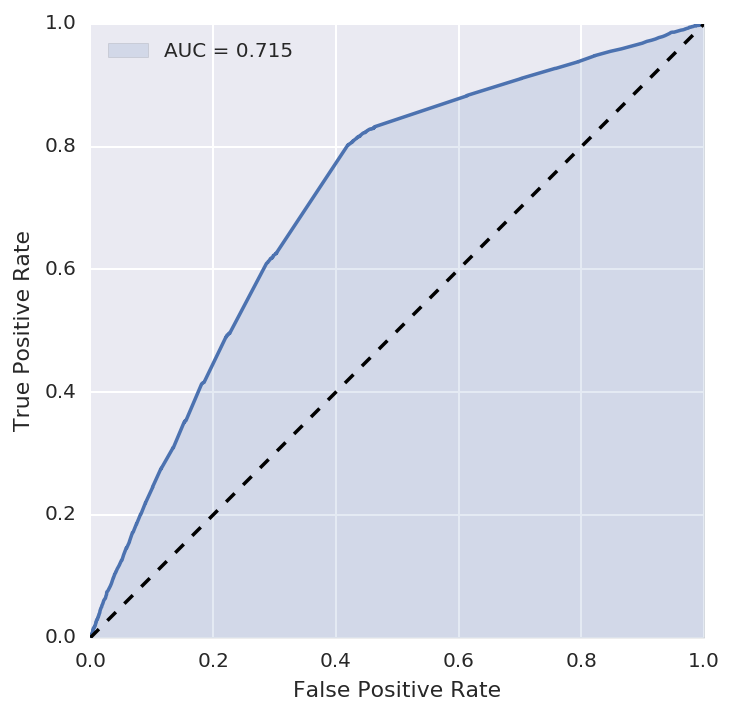
\includegraphics[width=.49\textwidth]{figures/bayes/roc_sms.png}
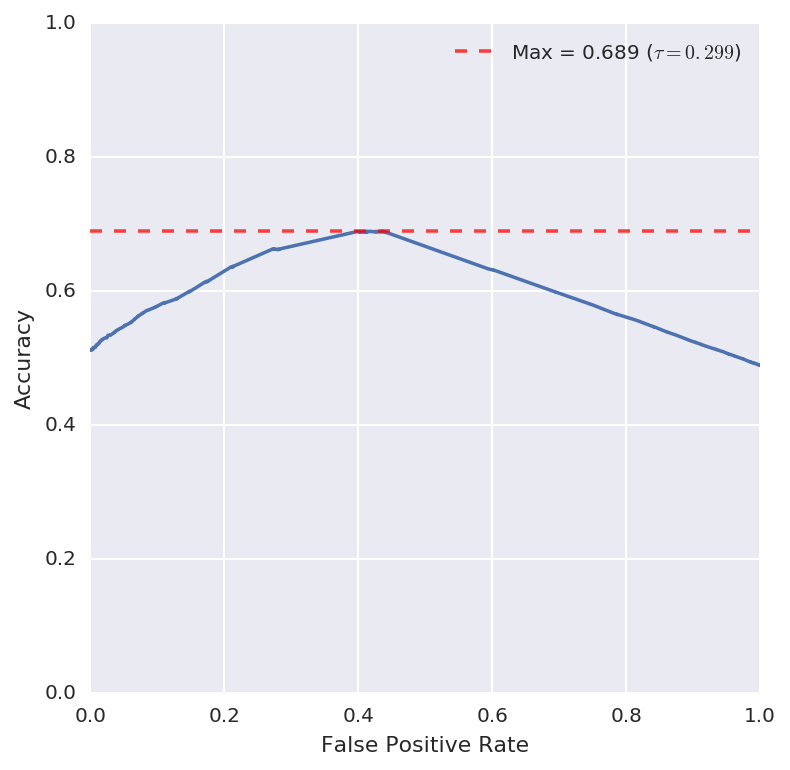
\includegraphics[width=.49\textwidth]{figures/bayes/accuracy_sms.png}
\end{center}

Since the total amount of SMS is much lower than the amount of calls, the peaks of the result of the \emph{Inverse Cumulative Functions} of the \emph{Beta Distribution} applied on $\Upsilon^{\sms}$ that happen with the majority of users that have few of both are located closer to the center than in Section~\ref{subsec:call_infer} and Section~\ref{subsec:time_infer}. This makes some interesting cases if $\varpi = \sms$ is chosen, since the distribution is different than in the other cases.

In particular, this gives an $\AUC = 0.715$, which is lower than both in the case of \emph{Calls} and \emph{Time}. Interesingly, the maximum \emph{Accuracy} at $\tau = 0.224$ is slightly higher than both of the other cases; this is probably a side-effect of the fact that $\left| \Upsilon^{\sms} \right| < \left| \Upsilon^{\calls} \right|$.

Additionally, $\FPR = 123$, $\Precision = 123$, $\Recall = 123$, $F_1 = 123$, and $F_4 = 123$. \todo{Fill these values.}

\subsubsection{Inferring by Contacts}
\label{subsec:contacts_infer}

\begin{center}
\includegraphics[width=\textwidth]{figures/bayes/hist_contacts.png}
\includegraphics[width=.49\textwidth]{figures/bayes/roc_contacts.png}
\includegraphics[width=.49\textwidth]{figures/bayes/accuracy_contacts.png}
\end{center}

When $\varpi = \contacts$ it's possible to get a pattern similar to the one shown in Section~\ref{subsec:sms_infer} when $\varpi = \sms$, where the majority of users have relatively few contacts and the peaks in the histogram. Additionally, since the total amount of contacts is logarithmically distributed (as shown in Figure~\ref{fig:contact_distribution}), and people with \emph{High Income} tend to have more contacts in general, there peaks are clustered in areas with low $p_v$ (where the majority of calls are made to \emph{Low Income} users), near the middle (where the calls are mostly equally distributed), but not at high $p_v$; this last section would belong to the few users with many calls to \emph{High Income} users.

Using this method it's possible to find that $\AUC = 0.742$, which is higher than all the other methods presented in Section~\ref{subsec:algorithm_performance}. Additionally, when selecting $\tau = 0.224$, $\Accuracy = 0.691$ which is higher than the maximum \emph{Accuracy} in all other methods. These metrics, combined with the fact that $\Upsilon$ contains every user in the \emph{Testing Set}, result in the fact that $\varpi = \contacts$ is uambiguously the best way to classify the data for the algorithm. Additionally, $\FPR = 123$, $\Precision = 123$, $\Recall = 123$, $F_1 = 123$, and $F_4 = 123$.

\subsection{Algorithm Performance of Users with at least 3 Contacts}

The algorithm tends to be a better predictor of the \emph{Socioeconomic Level} for users with high amount of information on the graph $G$, namely that the amount of users in their neighbourhood that also belong to $B$ is big.

In this section, we run the \emph{Bayesian Algorithm} for the subset of the users presented in Equation~\ref{eq:3contacts}, which restrict the users in the \emph{Testing Set} to only those who have at least 3 contacts. This would allow us to have better metrics in the dataset, at the expense of a much smaller Universe of users for which the algorithm could be applied. Additionally, Table~\ref{tab:3contacts} shows the sizes of the \emph{Testing Sets} used in a manner similar to Table~\ref{tab:partition_numbers}.

\begin{equation}
\label{eq:3contacts}
\begin{gathered}
I = \left\{ \upsilon \in \Upsilon \mid \contacts^{high}_{\upsilon} + \contacts^{\low}_{\upsilon} > 3 \right\} \\
I^{\calls} = \Upsilon^{\calls} \cap I
\end{gathered}
\end{equation}

\begin{table}
\centering
\begin{tabular}{l r r r c}
\toprule
Set & Total Size & High Income & Low Income & Ratio \\
\midrule
$I$ & \num{7932} & \num{4637} & \num{3295} & \num{0.258} \\
$I^{\calls}$ & \num{7910} & \num{4627} & \num{3283} & \num{0.214} \\
\bottomrule
\end{tabular}
\caption{Amount of users in the \emph{Testing Set} after trimming it several to only have users with at least 3 contacts.}
\label{tab:3contacts}
\end{table}

The same procedure applied in Section~\ref{subsec:calls_infer} and Section~\ref{subsec:contacts_infer} will be applied to this data.

\subsubsection{Inferring by Calls on Users with at least 3 Contacts}

\begin{center}
\includegraphics[width=\textwidth]{figures/bayes/3contacts/hist_calls.png}
\includegraphics[width=.49\textwidth]{figures/bayes/3contacts/roc_calls.png}
\includegraphics[width=.49\textwidth]{figures/bayes/3contacts/accuracy_calls.png}
\end{center}

Using $I^{\calls} \subseteq \Upsilon^{\calls}$ and $\varpi = \calls$ results in a predictor where both the \emph{Area Under the Curve} and the \emph{Accuracy} are higher than in all predictors that use every possible user. However, this data predicts less users and is strictly worse than the one predicting by Contacts presented in the following section.

\subsubsection{Inferring by Degree on Users with at least 3 Contacts}

\begin{center}
\includegraphics[width=\textwidth]{figures/bayes/3contacts/hist_contacts.png}
\includegraphics[width=.49\textwidth]{figures/bayes/3contacts/roc_contacts.png}
\includegraphics[width=.49\textwidth]{figures/bayes/3contacts/accuracy_contacts.png}
\end{center}

This dataset results in the best possible predictor for a reasonable subset of the users. Both the \emph{Area Under the Curve} and the \emph{Accuracy} are higher than for all other predictors: $\AUC = 0.829$, $\Accuracy = 0.766$, $\FPR = 123$, $\TPR = 123$, $\Precision = 123$, $\Recall = 123$, $F_1 = 123$, and $F_4 = 123$.

All of those values are considerably better than any other predictor in this page at the cost of using only a small subset of the possible users. This is interesing as it's exactly the same subset as the one used in~\cite{fixmanasonam2016}, and it scores significantly higher in all the metrics.


\bibliography{bibliography/sna}{}

\end{document}
